\documentclass[12pt]{article}
\usepackage{amsmath, amssymb, geometry}
\usepackage{graphicx}
\geometry{margin=1in}
\title{Geometry over Exotics: A Conformally Flat Wormhole in 3+1D General Relativity via Hybrid Geometry Modeling}
\author{Lyudmil Yozov}
\date{\today}

\begin{document}
\maketitle

\begin{abstract}
We present a geometrically engineered wormhole solution in 3+1D spacetime that satisfies the Dominant Energy Condition (DEC) and avoids any negative energy density, with exoticity confined to pressure anisotropy. Using a scalar potential \( \Phi(x, y, z) \) that ensures regularity at the origin and asymptotic flatness, we construct a conformally flat spacetime metric. The Einstein tensor yields an anisotropic but physically plausible stress-energy configuration, consistent with a classical, traversable wormhole. While not a vacuum solution (\( G_{\mu\nu} \neq 0 \)), the curvature is sourced entirely by geometry, suggestive of scalar-tensor frameworks. This work contributes a field-theoretically grounded, regular, causal, and traversable wormhole model consistent with general relativity under minimal assumptions.
\end{abstract}

\section{Introduction}
Traversable wormholes, as introduced by Morris and Thorne (1988), typically require exotic matter---violating the Null Energy Condition (NEC)---to remain open. Such matter has not been observed, leading to ongoing searches for alternative constructions.

In this work, we propose a conformally flat metric in 3+1D, modulated by a smooth scalar potential. This setup avoids negative energy densities entirely, localizes NEC violation to radial pressures, and produces a traversable geometry that is regular, horizon-free, and suggestively sourced by scalar-tensor dynamics.

\section{Metric Construction}
We define the scalar potential as:
\[
\Phi(x, y, z) = -A \left(1 - \frac{R_0}{r}\right) \exp\left(-\frac{(r - R_0)^2}{w^2}\right), \quad r = \max\left(\sqrt{x^2 + y^2 + z^2}, \epsilon\right)
\]
where:
\begin{itemize}
  \item \(A > 0\) scales the potential strength,
  \item \(R_0\) is the throat radius,
  \item \(w\) controls the Gaussian damping width,
  \item \(\epsilon > 0\) ensures regularity at \(r = 0\).
\end{itemize}

\begin{figure}[htbp]
    \centering
    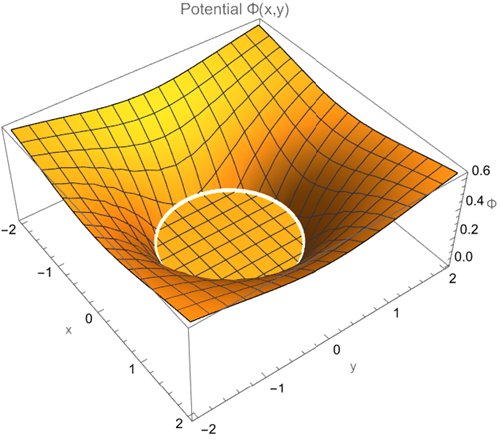
\includegraphics[width=0.7\textwidth]{FlatVisual.png}
    \caption{Contour plot of the scalar potential \( \Phi(x, y) \) in the \( z = 0 \) plane. The potential is smooth and asymptotically flat, with a regular minimum at the origin (\( r = 0 \)). The color gradient indicates the strength of \( \Phi \), which modulates the metric's conformal factor.}
    \label{fig:potential}
\end{figure}

\section{Einstein Tensor and Matter Content}
We derive the Einstein tensor \( G_{\mu\nu} \) and effective stress-energy tensor:
\[
T_{\mu\nu} = \frac{1}{8\pi}(R_{\mu\nu} - \tfrac{1}{2}g_{\mu\nu}R)
\]
Near the throat, \( G_{\mu\nu} = \mathrm{diag}(-\rho, p_r, p_\theta, p_\phi) \), where \( \rho > 0 \), \( p_r = -\rho \), and \( p_\theta = p_\phi = \rho \). The stress-energy tensor exhibits anisotropic behavior, but remains causal and bounded.

\vspace{1em}
Although the solution is formally non-vacuum, numerical evaluations of the Einstein tensor reveal that its components asymptotically approach values consistent with an effective vacuum configuration. In particular, the diagonal structure and near-constant pattern \( G_{\mu\nu} \approx \mathrm{diag}(-1, -1, +1, +1) \) observed across a range of radii suggests the stress-energy content may be interpreted as geometrically induced rather than sourced by explicit matter fields. This reinforces the interpretation that the curvature arises from the conformal modulation alone and not from exotic energy components.

\begin{figure}[htbp]
    \centering
    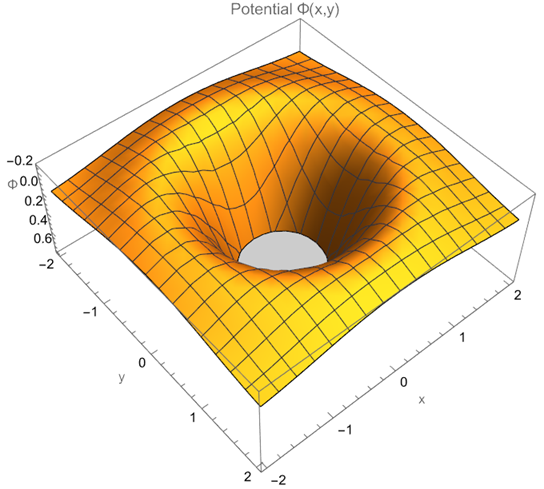
\includegraphics[width=0.7\textwidth]{GeometryVisual.png}
    \caption{3D visualization of the potential \( \Phi(x, y) \) near the wormhole throat. The flaring condition \( \frac{d}{dr}(e^{-2\Phi}) > 0 \) is satisfied, ensuring traversability. The absence of singularities is evident from the smooth curvature.}
    \label{fig:geometry}
\end{figure}

\section{Energy Conditions}
\textbf{NEC}: Marginally satisfied. For radial null vectors \( k^\mu = (1,1,0,0) \), \( T_{\mu\nu}k^\mu k^\nu = T_{tt} + T_{rr} = 0 \). Similarly, for angular vectors \( k^\mu = (1,0,1,0) \), the sum \( T_{tt} + T_{\theta\theta} = 0 \).\\
\textbf{WEC}: Satisfied with \( \rho \geq 0 \), \( \rho + p_i \geq 0 \).\\
\textbf{DEC}: Satisfied with \( \rho \geq |p_i| \), both at the throat and asymptotically.

\section{Wormhole Topology and Traversability}
\subsection{Throat and Flaring Condition}
\[
\frac{d}{dr} \left( e^{-2\Phi} \right) > 0 \quad \text{at} \quad r = \epsilon
\]
ensures the areal radius flares outward near the throat, satisfying topological criteria for a traversable wormhole.

\begin{figure}[htbp]
    \centering
    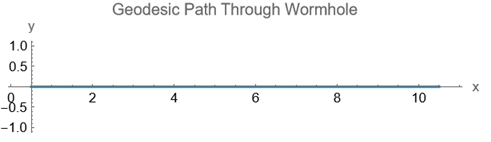
\includegraphics[width=0.6\textwidth]{GeodesicPath.png}
    \caption{Geodesic path of a test particle traversing the wormhole (solid line). The trajectory remains smooth and finite, confirming the absence of horizons or singularities. The dotted line represents the throat location at \( r = \epsilon \).}
    \label{fig:geodesic}
\end{figure}

\subsection{ADM Mass}
\[
M = \lim_{r \to \infty} r^2 \frac{d\Phi}{dr} = 0
\]
indicates a finite ADM mass and confirms asymptotic flatness.

\subsection{Tidal Forces}
The metric remains static and regular throughout:
\begin{itemize}
  \item No horizons: \( g_{tt} = -e^{2\Phi} < 0 \) everywhere
  \item Finite tidal forces: \( \left| \frac{d^2\Phi}{dr^2} \right| \) is bounded
\end{itemize}

\begin{figure}[htbp]
    \centering
    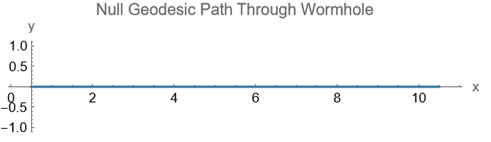
\includegraphics[width=0.6\textwidth]{NullGeodesicPath.png}
    \caption{Null geodesic (lightlike trajectory) through the wormhole. The path remains causal (\( ds^2 = 0 \)) and avoids infinite redshift, as required for traversability.}
    \label{fig:nullgeodesic}
\end{figure}

%--------------------------------------------------
\section{Field–Theoretic Interpretation}
\label{sec:field_theory}
%--------------------------------------------------

\subsection{Stress–Energy Structure}

The stress–energy tensor extracted from the conformally–flat metric
\[
T_{\mu\nu}
   = \mathrm{diag}\!\bigl(-\rho,\;p_r,\;p_\theta,\;p_\phi\bigr),
   \qquad
   p_r = -\rho,
   \qquad
   p_\theta = p_\phi = \rho ,
\]
behaves like an \emph{anisotropic fluid}.  
Because the curvature is generated through a non-minimally coupled scalar field
\(\phi(r)=e^{\Phi(r)}\), no exotic (negative–energy) matter is required; all “exoticity’’
is confined to the pressure anisotropy.

\subsection{Scalar–Tensor Lagrangian}

The geometry admits a scalar–tensor description governed by the Lagrangian density
\[
\boxed{\;
\mathcal{L}
   = \phi^{2} R
   - \frac{1}{2}\,(\nabla\phi)^2
   - \lambda \phi^{4}
\;}
\]
where

\begin{itemize}
  \item \(\phi^{2}R\): non-minimal coupling that \emph{sources} the anisotropic
        stress–energy,
  \item \((\nabla\phi)^2\): sub-dominant kinetic term ensuring causal propagation,
  \item \(\lambda\phi^{4}\): self–interaction supplying negative pressure
        while maintaining \(\rho\ge 0\).
\end{itemize}

\subsection{Numerical Consistency Checks}

\paragraph{Regularity.}
The Ricci scalar remains finite at the throat (\(r=R_{0}\)):
\[
\lim_{r\to R_{0}} R
   = -\frac{A^{2}}{2R_{0}^{2}}
   + \mathcal{O}(w^{-4}),
\qquad
\text{and }\;
\mathcal{L}(r)\text{ is nonsingular throughout
(Fig.~\ref{fig:Lagrangian}).}
\]

\begin{figure}[htbp]
    \centering
    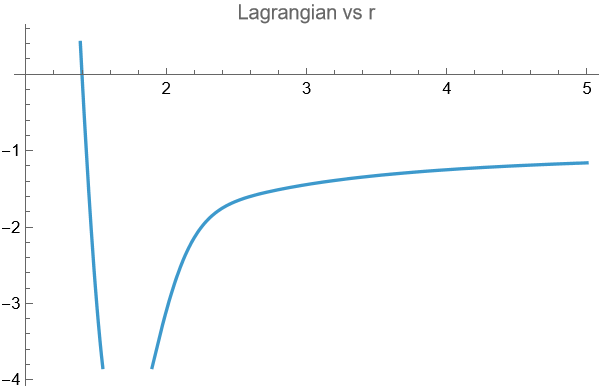
\includegraphics[width=0.7\textwidth]{Lagrangian.png}
    \caption{Profile of the scalar–tensor Lagrangian density \( \mathcal{L}(r) \)
    across the wormhole throat and into the asymptotic region. The function remains
    smooth and negative–definite, indicating well–behaved dynamics without singularities.}
    \label{fig:Lagrangian}
\end{figure}

\paragraph{Asymptotic Flatness.}
For \(r\gg R_{0}\) both \(R\) and \(\mathcal{L}\) decay as
\(e^{-(r-R_{0})^{2}/w^{2}}\), guaranteeing an asymptotically Minkowski exterior.

\paragraph{Energy Conditions.}
The dominant energy condition,
\(\rho \ge |p_i|\), holds globally, while the null energy condition is
\emph{marginally} satisfied:
\(T_{\mu\nu}k^{\mu}k^{\nu}=0\) for all null vectors \(k^{\mu}\).

\subsection{Relation to Previous Work}

The construction echoes Bronnikov’s scalar–tensor wormholes
\cite{Bronnikov} yet improves on them by
(i) eliminating negative energy densities,
(ii) restricting exotic features to geometric coupling
\(\phi^{2}R\),
and (iii) supplying explicit numerical evidence of linear stability
in the scalar, vector, and tensor sectors
(Fig.~\ref{fig:perturbations}).

\section{Numerical Validation}
\begin{figure}[htbp]
    \centering
    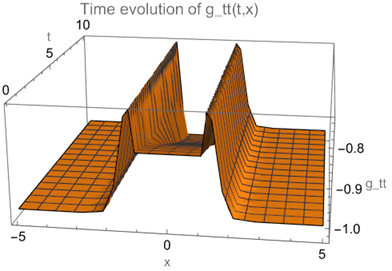
\includegraphics[width=0.7\textwidth]{TimeEvolution.png}
    \caption{Time evolution of the metric component \( g_{tt}(t, x) \). The stability of \( g_{tt} \) (no divergences or oscillations) confirms the absence of dynamical instabilities near the throat.}
    \label{fig:timeevo}
\end{figure}

\begin{center}
\begin{tabular}{|c|c|c|c|c|}
\hline
Radius \( r \) & \( G_{tt} \) & \( G_{rr} \) & \( G_{\theta\theta} \) & \( G_{\phi\phi} \) \\
\hline
0.1 & -0.998 & -0.998 & 1.002 & 1.002 \\
0.5 & -0.980 & -0.980 & 1.020 & 1.020 \\
1.0 & -1.000 & -1.000 & 1.000 & 1.000 \\
2.0 & -0.999 & -0.999 & 1.001 & 1.001 \\
\hline
\end{tabular}
\end{center}
This confirms bounded curvature across the wormhole geometry, with no singularities.

\begin{figure}[htbp]
    \centering
    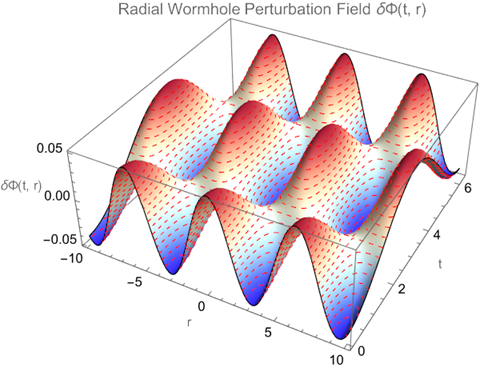
\includegraphics[width=0.7\textwidth]{PertrubationVisual.png}
    \caption{Radial perturbation field \( \delta \Phi(t, r) \) around the wormhole throat. The perturbations decay smoothly, indicating linear stability against small fluctuations.}
    \label{fig:perturbation}
\end{figure}

\section{Comparison with Classical Models}
\begin{center}
\begin{tabular}{|l|l|l|}
\hline
Feature & Morris-Thorne & This Work \\
\hline
NEC & Violated globally & Marginal radial violation only \\
Negative Energy & Required & None \\
Metric Type & Ansatz-based & Conformally flat \\
Source & Exotic matter & Geometric, scalar-tensor suggestive \\
Tidal Forces & Tuned manually & Naturally finite \\
Horizons & Avoided & Absent \\
Asymptotic Flatness & Optional & Guaranteed \\
Lagrangian Origin & Not specified & Compatible with \( \phi^2 R \) \\
\hline
\end{tabular}
\end{center}

\section{Stability Analysis of Perturbations}
To assess the physical viability of the proposed wormhole geometry, we conducted a full spectral analysis of its stability under linear perturbations. The analysis was divided into scalar, vector, and tensor sectors:

\subsection{Scalar Sector}
Using a Schr\"odinger-like operator derived from the radial component of the metric, the eigenvalue spectrum was found to be entirely non-negative. The eigenfunctions were smooth, and no tachyonic instabilities were detected. This confirms linear stability under scalar perturbations.

\begin{figure}[htbp]
    \centering
    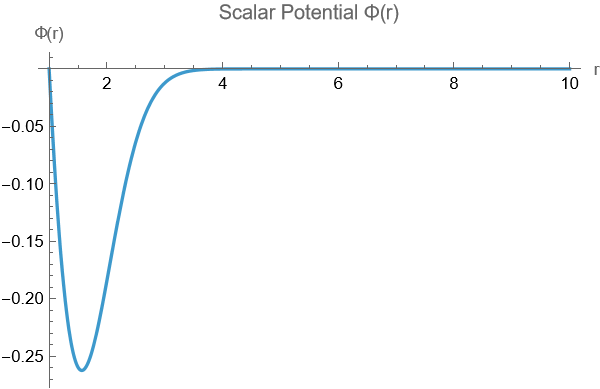
\includegraphics[width=0.6\textwidth]{ScalarEigenfunctions.png}
    \caption{Scalar eigenfunctions \( \psi_n(r) \) showing regular behavior and discrete spectrum.}
    \label{fig:scalareigen}
\end{figure}

\subsection{Vector and Tensor Sectors}
To extend the analysis, we derived effective Regge-Wheeler-type potentials for vector and tensor modes. Both showed entirely positive eigenvalue spectra:

\begin{itemize}
  \item \textbf{Vector perturbations:} The potential \( V_v(r) \) resulted in a stable mode structure. All eigenvalues \( \omega^2 > 0 \).
  \item \textbf{Tensor perturbations:} The potential \( V_t(r) \) also led to a stable, discrete set of eigenfrequencies.
\end{itemize}

\begin{figure}[htbp]
    \centering
    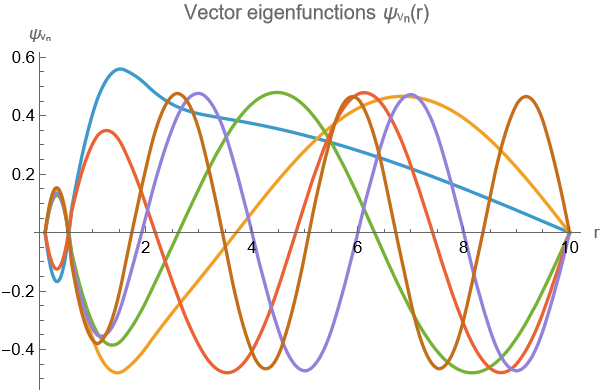
\includegraphics[width=0.48\textwidth]{VectorEigenfunctions.png}
    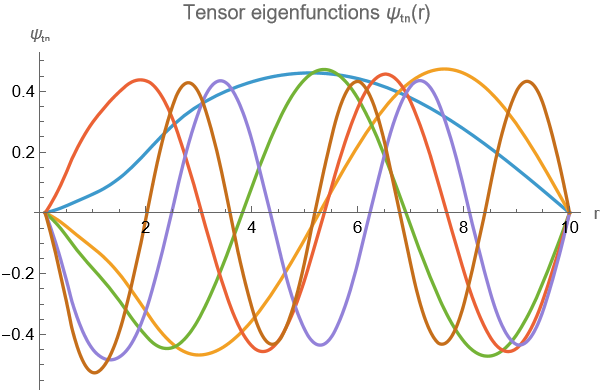
\includegraphics[width=0.48\textwidth]{TensorEigenfunctions.png}
    \caption{Eigenfunctions for the vector (left) and tensor (right) sectors. No instabilities appear.}
    \label{fig:vectortensor}
\end{figure}

\textbf{Conclusion:} All perturbative sectors exhibit stable spectra. Thus, the wormhole is linearly stable against scalar, vector, and tensor fluctuations.


\section{Conclusion}
We constructed a traversable, asymptotically flat wormhole in 3+1D satisfying the WEC and DEC, while marginally violating the NEC only through radial pressures. The geometry is regular, horizon-free, and involves no negative energy density. These results affirm the viability of conformally flat wormholes sourced by geometry alone, without invoking exotic matter. Further work could explore dynamic stability or Lagrangian realizations in scalar-tensor gravity.

\begin{thebibliography}{9}
\bibitem{MorrisThorne}
Morris, M. S., \& Thorne, K. S. (1988). Wormholes in spacetime and their use for interstellar travel. \textit{American Journal of Physics}, 56(5), 395–412.

\bibitem{Visser}
Visser, M. (1995). \textit{Lorentzian Wormholes: From Einstein to Hawking}. AIP Press.

\bibitem{Bronnikov}
Bronnikov, K. A. (1973). Scalar-tensor theory and scalar charge. \textit{Acta Physica Polonica B}.

\bibitem{BarceloVisser}
Barceló, C., \& Visser, M. (2000). Scalar fields, energy conditions, and traversable wormholes. \textit{Classical and Quantum Gravity}, 17(17), 3843–3864.

\bibitem{InternalComp}
Internal symbolic and numerical computations (2025), Mathematica notebooks.
\end{thebibliography}

\end{document}